\section{Durchführung}
\label{sec:Durchführung}

\subsection{Versuchsaufbau}
\label{sec:Versuchsaufbau}
%\begin{figure}
%	\centering
%	\caption{Schematische Darstellung des Versuchsaufbaus \cite{anleitung}.}
%	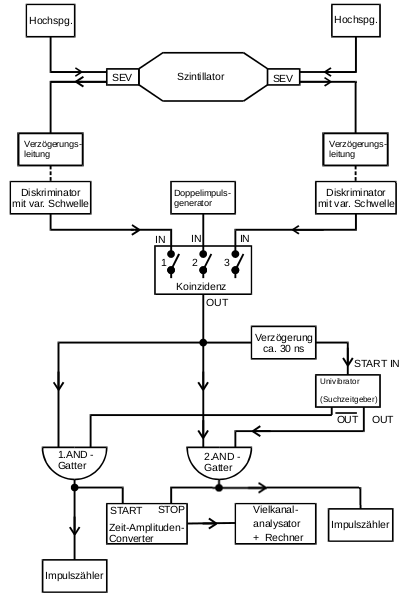
\includegraphics{Bilder/aufbau.png}
%	\label{fig:aufbau}
%\end{figure}
%
%\begin{figure}
%	\centering
%	\caption{Schematische Darstellung der Quelle zur Erzeugung radioaktiven Isotopen \cite{anleitung}.}
%	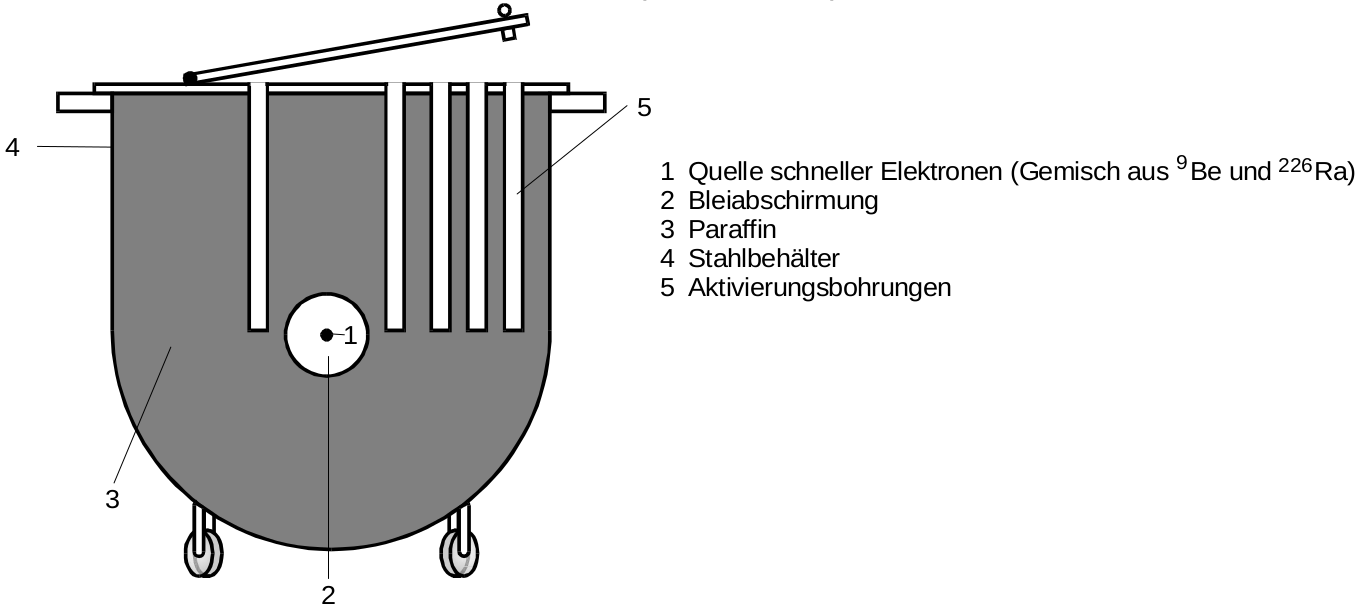
\includegraphics{content/toepfchen.png}
%	\label{fig:kochen}
%\end{figure}
%
Der Versuchsaufbau -- wie in Abbildung \ref{fig:aufbau} dargestellt -- besteht im Wesentlichen 
aus einem zerfallenden radioaktiven Isotop und einem Geiger-Müller-Zählrohr, welches die 
zerfallenden Kerne misst.
Das Geiger-Müller-Zählrohr ist entspricht einer mit Gas gefüllten Röhre. Trifft ein $\beta$-
oder $\gamma$- Teilchen auf ein Gasteilchen wird dieses ionisiert und kann aufgrund einer
anliegenden Spannung an der Röhre gemessen werden.
Dabei werden die gemessenen Zerfälle pro Messzeitintervall, welches am Zeitgeber einstellbar 
ist, an den Zählern 1 und 2 angezeigt. Nach jedem Messvorgang wird der Zähler umgeschaltet und 
der vorherige Wert auf dem aktuellen Zähler wird überschrieben. Der Versuchsaufbau ist mit
einer Blei-Abschirmung ausgestattet um die radioaktive Strahlung abzuschirmen.

Zur Erzeugung der radioaktiven Isotope wird das Objekt in Abbildung \ref{fig:kochen} verwendet.
Hierbei werden stabile Kerne mit niederenergetischen Neutronen beschossen. 
Da die Neutronen ihre Energie durch elastische Stöße an die Kerne übergeben und die maximale
Energie bei gleichen Massen der Stoßpartner erreicht wird, werden die Neutronen in einem 
Paraffinmantel gebremst, bis sie die optimale Energie besitzen.


\subsection{Versuchsbeschreibung}
\label{sec:Versuchsbeschreibung}

Eine halbe Stunde vor der Messung wird der Ofen eingeschaltet, um den richtigen
Dampfdruck zu erzeugen.
Daraufhin werden die optischen Objekte justiert, sodass die Intensität maximal wird.
Dafür müssen an der Kontrollvorrichtung alle "GAIN"-Knöpfe auf "1" gestellt werden. 
Nach der Justierung wird eine schwarze Decke über den Aufbau gelegt, um externes Licht 
abzuschirmen. 

Als zweiter Schritt wird der gesamte Aufbau in Nord-Süd-Richtung gedreht, damit 
die Horizontalkomponente des Erdmagnetfeldes entweder parallel oder antiparallel 
zur Horizontalfeldspule ausgerichtet ist.
Dann wird die vertikale Komponente des Erdmagnetfeldes mit der Vertikalfeldspule 
kompensiert. Hierzu soll auf dem Oszilloskop ein möglichst scharfer Peak zu erkennen sein.
Dies geschieht mit abwechselnder Justierung der Position des Aufbaus in Nord-Süd-Richtung und 
dem Einstellen des Spulenstroms der Vertikalfeldspule.
Hierfür muss der untere Schalter für die Sweep-Spule auf "CONTINUOUS" und der Obere
auf "START" gestellt werden. Weiterhin muss für beide Kanäle am Oszilloskop DC-Kopplung
eingestellt sein. Der "GAIN" soll auf 20, der "GAIN MULTIPLIER" auf x10 und der "METER
MULTIPLIER" soll auf x2 geschaltet sein. Der Wert für den eingestellten Spulenstroms
wird notiert und nicht mehr verändert.

Nun wird das gesamte Horizontalfeld in Abhängigkeit von den Resonanzfrequenzen der beiden 
Rubidium-Isotope gemessen. Hierfür wird die Frequenz (Sinus-Spannung) im Bereich
von $\SI{100}{\kilo\hertz}-\SI{1}{\mega\hertz}$ in $\SI{100}{\kilo\hertz}$-Schritten
variiert.
Für höhere Frequenzen (ab $\SI{200}{\kilo\hertz}$) wird ein zusätzliches Horizontalfeld 
benötigt, damit die Resonanzen im Sweet-Feld-Bereich liegen.
Es werden jeweils für die Frequenzen die beiden Resonanzen notiert. Der Strom bei dem 
die Resonanzen auftreten kann am Potentiometer abgelesen werden, wobei eine Umdrehung
$\SI{0,1}{\ampere}$ entspricht.
